\section{Definitions}

A complex number $z$ is generally written in the form $z=a+bi$ where $a$ and $b$ are real numbers and $i$, called the imaginary unit, has the property that $i^2=-1$. The real numbers $a$ and $b$ are called the real and imaginary parts of $z=a+bi$, respectively.

The complex conjugate of $z$ is denoted by $\bar{z}$; it is defined by $\overline{a+bi}=a-bi$. Thus, $a+bi$ and $a-bi$ are conjugates of each other.

\section{Equality of Complex Numbers}

$a+bi=c+di$ if and only if $a=c$ and $b=d$

\section{Arithmetic of Complex Numbers}

$$(a+bi)+(c+di)=(a+c)+(b+d)i$$

$$(a+bi)-(c+di)=(a-c)+(b-d)i$$

$$(a+bi)(c+di)=(ac-bd)+(ad+bc)i$$

$$\dfrac{a+bi}{c+di}=\dfrac{(a+bi)(c-di)}{(c+di)(c-di)}=\dfrac{ac+bd}{c^2+d^2}+\dfrac{bc-ad}{c^2+d^2}i$$

\section{Polar Form of Complex Numbers}

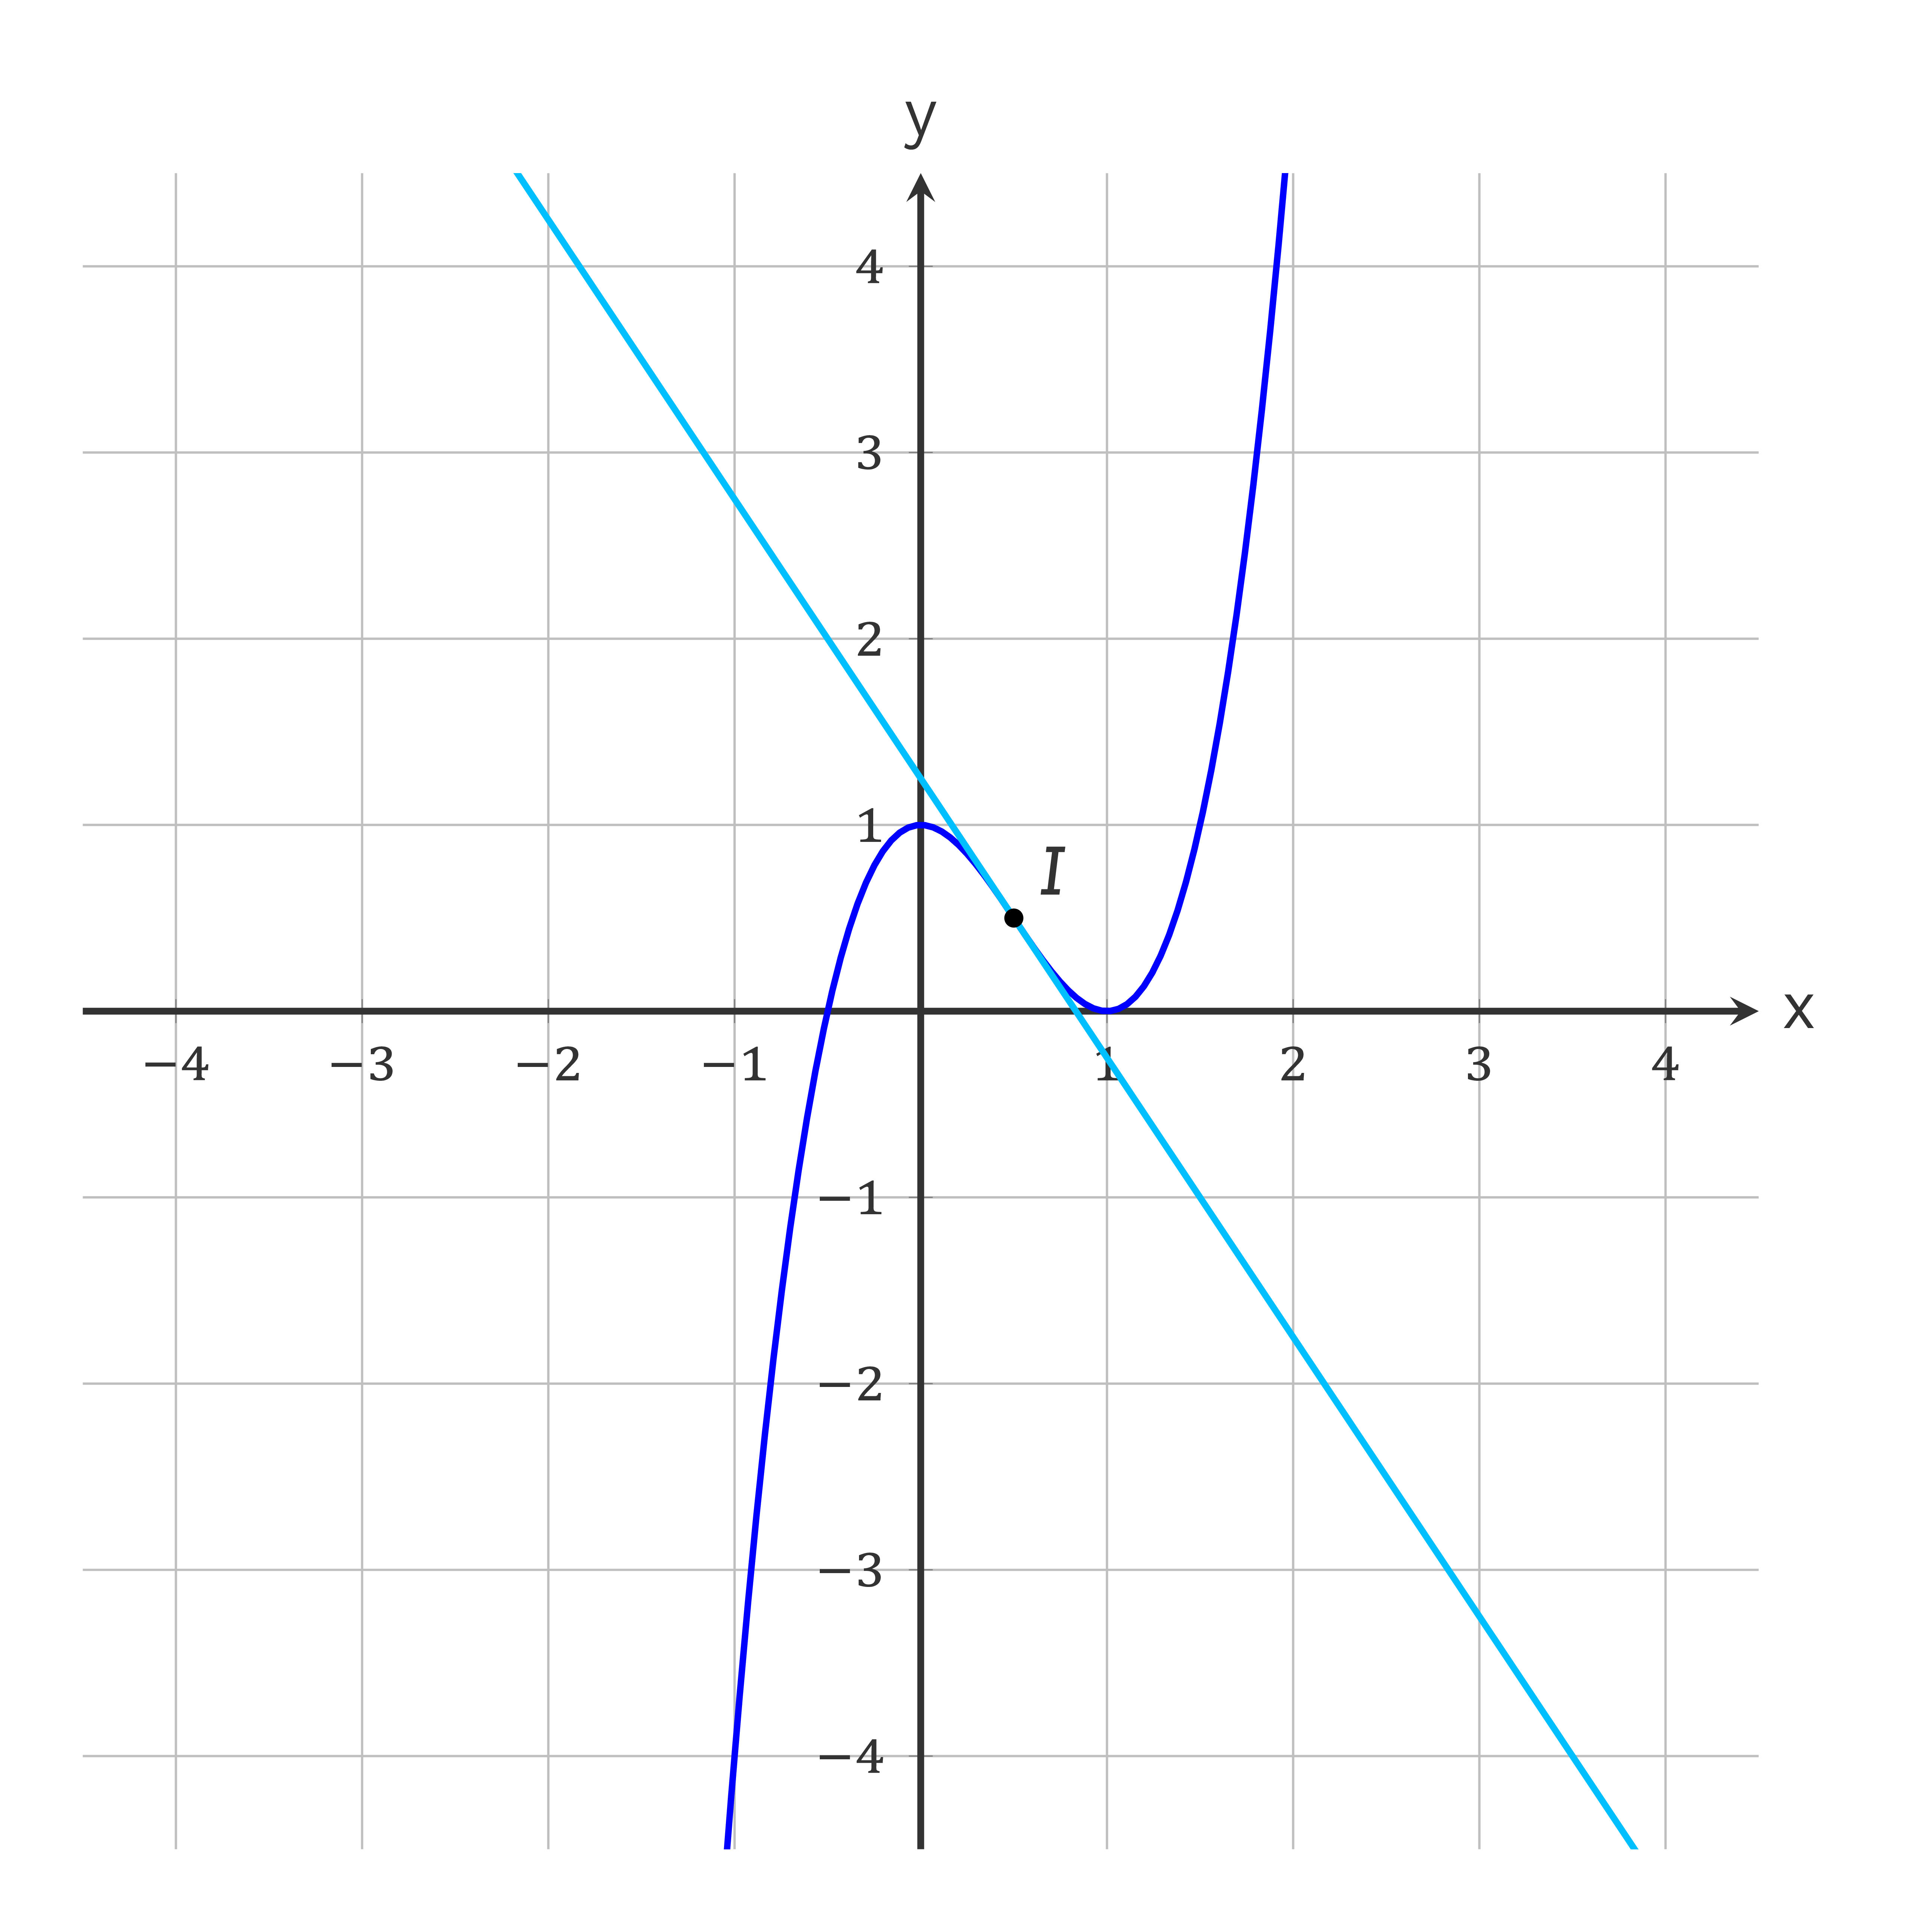
\includegraphics{graph}

The point $P(x,y)$ represents the complex number $z=x+iy$. The point $P$ can also be represented by polar coordinates $(r,\theta)$. Since $x=r\cos \theta$ and $y=r\sin \theta$, we have
$$z=x+iy=r(\cos \theta+i\sin \theta)$$
called the Polar Form of the complex number. We often call $r=|z|=\sqrt{r^2+y^2}$ the modulus and $\theta$ the amplitude of $z=x=iy$.

\section{Multiplication and Division of Complex Numbers in Polar Form}

If $z_1=r_1\left( \cos \theta_1 +i\sin \theta_1\right)$ and $z_2=r_2\left( \cos \theta_2 +i\sin \theta_2\right)$ then
$$\begin{aligned} 
&z_1z_2=r_1r_2\left[\cos\left( \theta_1+\theta_2 \right)+i\sin\left( \theta_1+\theta_2 \right) \right] \\
&\dfrac{r_1}{r_2}=\dfrac{r_1}{r_2}\left[\cos\left(\theta_2-\theta_1\right)+i\sin \left(\theta_2-\theta_1 \right)\right]
\end{aligned}$$

\section{De Moivre's Theorem}

If $z=r\left( \cos \theta + i\sin \theta \right)$ and $n$ is a positive integer, then 
$$z^n=r^n\left( \cos n\theta + i\sin \theta \right)$$

\section{Roots of a Complex Number}

Let $z=r\left( \cos \theta + i\sin \theta \right)$ and let $n$ be a positive integer. Then $z$ has the $n$ distinct nth roots
$$w_k=r^{1/n}\left[ \cos \left( \dfrac{\theta + 2k\pi}{n} \right) + i\sin \left( \dfrac{\theta + 2k\pi}{n} \right) \right]$$
Where $k=1,2,3,..., (n-1)$.



